\documentclass{book}
\usepackage[a4paper,top=2.5cm,bottom=2.5cm,left=2.5cm,right=2.5cm]{geometry}
\usepackage{makeidx}
\usepackage{natbib}
\usepackage{graphicx}
\usepackage{multicol}
\usepackage{float}
\usepackage{listings}
\usepackage{color}
\usepackage{ifthen}
\usepackage[table]{xcolor}
\usepackage{textcomp}
\usepackage{alltt}
\usepackage{ifpdf}
\ifpdf
\usepackage[pdftex,
            pagebackref=true,
            colorlinks=true,
            linkcolor=blue,
            unicode
           ]{hyperref}
\else
\usepackage[ps2pdf,
            pagebackref=true,
            colorlinks=true,
            linkcolor=blue,
            unicode
           ]{hyperref}
\usepackage{pspicture}
\fi
\usepackage[utf8]{inputenc}
\usepackage{mathptmx}
\usepackage[scaled=.90]{helvet}
\usepackage{courier}
\usepackage{sectsty}
\usepackage{amssymb}
\usepackage[titles]{tocloft}
\usepackage{doxygen}
\lstset{language=C++,inputencoding=utf8,basicstyle=\footnotesize,breaklines=true,breakatwhitespace=true,tabsize=4,numbers=left }
\makeindex
\setcounter{tocdepth}{3}
\renewcommand{\footrulewidth}{0.4pt}
\renewcommand{\familydefault}{\sfdefault}
\hfuzz=15pt
\setlength{\emergencystretch}{15pt}
\hbadness=750
\tolerance=750
\begin{document}
\hypersetup{pageanchor=false,citecolor=blue}
\begin{titlepage}
\vspace*{7cm}
\begin{center}
{\Large Oblig 3 }\\
\vspace*{1cm}
{\large Generated by Doxygen 1.8.3.1}\\
\vspace*{0.5cm}
{\small Mon Mar 18 2013 17:17:37}\\
\end{center}
\end{titlepage}
\clearemptydoublepage
\pagenumbering{roman}
\tableofcontents
\clearemptydoublepage
\pagenumbering{arabic}
\hypersetup{pageanchor=true,citecolor=blue}
\chapter{Hierarchical Index}
\section{Class Hierarchy}
This inheritance list is sorted roughly, but not completely, alphabetically\-:\begin{DoxyCompactList}
\item \contentsline{section}{Element}{\pageref{d5/d50/class_element}}{}
\begin{DoxyCompactList}
\item \contentsline{section}{Num\-\_\-element}{\pageref{d8/d1c/class_num__element}}{}
\item \contentsline{section}{Text\-\_\-element}{\pageref{db/d3d/class_text__element}}{}
\end{DoxyCompactList}
\item \contentsline{section}{List}{\pageref{d1/d34/class_list}}{}
\item \contentsline{section}{localdb}{\pageref{db/db5/classlocaldb}}{}
\item \contentsline{section}{medicine}{\pageref{d3/d07/structmedicine}}{}
\item \contentsline{section}{person}{\pageref{d7/db3/classperson}}{}
\item \contentsline{section}{prescription}{\pageref{d0/dd9/classprescription}}{}
\item \contentsline{section}{substance}{\pageref{d3/df8/classsubstance}}{}
\item \contentsline{section}{userio}{\pageref{dc/ddf/classuserio}}{}
\end{DoxyCompactList}

\chapter{Class Index}
\section{Class List}
Here are the classes, structs, unions and interfaces with brief descriptions\-:\begin{DoxyCompactList}
\item\contentsline{section}{\hyperlink{class_element}{Element} }{\pageref{d5/d50/class_element}}{}
\item\contentsline{section}{\hyperlink{class_list}{List} }{\pageref{d1/d34/class_list}}{}
\item\contentsline{section}{\hyperlink{classlocaldb}{localdb} }{\pageref{db/db5/classlocaldb}}{}
\item\contentsline{section}{\hyperlink{structmedicine}{medicine} }{\pageref{d3/d07/structmedicine}}{}
\item\contentsline{section}{\hyperlink{class_num__element}{Num\-\_\-element} }{\pageref{d8/d1c/class_num__element}}{}
\item\contentsline{section}{\hyperlink{classperson}{person} }{\pageref{d7/db3/classperson}}{}
\item\contentsline{section}{\hyperlink{classprescription}{prescription} }{\pageref{d0/dd9/classprescription}}{}
\item\contentsline{section}{\hyperlink{classsubstance}{substance} }{\pageref{d3/df8/classsubstance}}{}
\item\contentsline{section}{\hyperlink{class_text__element}{Text\-\_\-element} }{\pageref{db/d3d/class_text__element}}{}
\item\contentsline{section}{\hyperlink{classuserio}{userio} }{\pageref{dc/ddf/classuserio}}{}
\end{DoxyCompactList}

\chapter{Class Documentation}
\hypertarget{class_element}{\section{Element Class Reference}
\label{d5/d50/class_element}\index{Element@{Element}}
}


Inheritance diagram for Element\-:\nopagebreak
\begin{figure}[H]
\begin{center}
\leavevmode
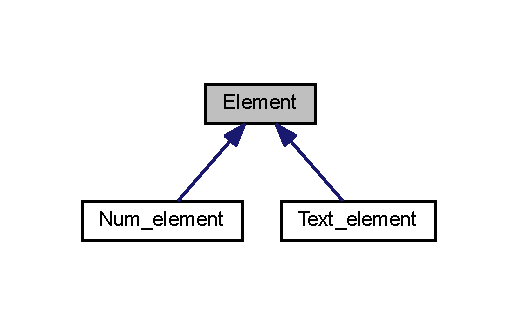
\includegraphics[width=249pt]{df/d0d/class_element__inherit__graph}
\end{center}
\end{figure}
\subsection*{Public Member Functions}
\begin{DoxyCompactItemize}
\item 
\hypertarget{class_element_a7e572183ea4b57781a9d896caaafbf2f}{char {\bfseries get\-\_\-type} ()}\label{d5/d50/class_element_a7e572183ea4b57781a9d896caaafbf2f}

\item 
\hypertarget{class_element_a07bbee15ca80992dec60254fac6b004e}{virtual int {\bfseries compare} (\hyperlink{class_element}{Element} $\ast$el)}\label{d5/d50/class_element_a07bbee15ca80992dec60254fac6b004e}

\item 
\hypertarget{class_element_a104b244ec65250b42d6d6713393684e0}{virtual void {\bfseries display} ()}\label{d5/d50/class_element_a104b244ec65250b42d6d6713393684e0}

\end{DoxyCompactItemize}
\subsection*{Friends}
\begin{DoxyCompactItemize}
\item 
\hypertarget{class_element_a8332d6f5b691636d30b5c7a91addf247}{class {\bfseries Num\-\_\-element}}\label{d5/d50/class_element_a8332d6f5b691636d30b5c7a91addf247}

\item 
\hypertarget{class_element_af2cc0329ecc045324a0815c7d55b79f5}{class {\bfseries Text\-\_\-element}}\label{d5/d50/class_element_af2cc0329ecc045324a0815c7d55b79f5}

\end{DoxyCompactItemize}


The documentation for this class was generated from the following files\-:\begin{DoxyCompactItemize}
\item 
list\-\_\-tool.\-h\item 
list\-\_\-tool.\-cpp\end{DoxyCompactItemize}

\hypertarget{class_list}{\section{List Class Reference}
\label{d1/d34/class_list}\index{List@{List}}
}
\subsection*{Public Member Functions}
\begin{DoxyCompactItemize}
\item 
\hypertarget{class_list_afd7e4e5bbb9551737d314733718443e3}{{\bfseries List} (listtype li)}\label{d1/d34/class_list_afd7e4e5bbb9551737d314733718443e3}

\item 
\hypertarget{class_list_a52c58a2f1cbbc8f6b5be599d36650b92}{int {\bfseries is\-\_\-empty} ()}\label{d1/d34/class_list_a52c58a2f1cbbc8f6b5be599d36650b92}

\item 
\hypertarget{class_list_a15316f30a5a14a6ab3cded1bbb3a7cf2}{int {\bfseries no\-\_\-of\-\_\-elements} ()}\label{d1/d34/class_list_a15316f30a5a14a6ab3cded1bbb3a7cf2}

\item 
\hypertarget{class_list_a0c68e2a53bf6f62b8776b6452e033285}{bool {\bfseries add} (\hyperlink{class_element}{Element} $\ast$el)}\label{d1/d34/class_list_a0c68e2a53bf6f62b8776b6452e033285}

\item 
\hypertarget{class_list_a140f49178e342df457c44cf5adcb4251}{\hyperlink{class_element}{Element} $\ast$ {\bfseries remove} ()}\label{d1/d34/class_list_a140f49178e342df457c44cf5adcb4251}

\item 
\hypertarget{class_list_a08d3e1577f17dc433376f822e3003b88}{\hyperlink{class_element}{Element} $\ast$ {\bfseries remove} (int no)}\label{d1/d34/class_list_a08d3e1577f17dc433376f822e3003b88}

\item 
\hypertarget{class_list_ac0808e64bb3ce2ee624c3c45c8db48d2}{\hyperlink{class_element}{Element} $\ast$ {\bfseries remove} (const char $\ast$t)}\label{d1/d34/class_list_ac0808e64bb3ce2ee624c3c45c8db48d2}

\item 
\hypertarget{class_list_aa80d82f65f222e774848aa845f4821a6}{\hyperlink{class_element}{Element} $\ast$ {\bfseries remove\-\_\-no} (int n)}\label{d1/d34/class_list_aa80d82f65f222e774848aa845f4821a6}

\item 
\hypertarget{class_list_a3a325ba9176f9f586c1813655cddcc90}{bool {\bfseries destroy} ()}\label{d1/d34/class_list_a3a325ba9176f9f586c1813655cddcc90}

\item 
\hypertarget{class_list_a2d3c6cfdadbadd2da665f807a6a059ea}{bool {\bfseries destroy} (int no)}\label{d1/d34/class_list_a2d3c6cfdadbadd2da665f807a6a059ea}

\item 
\hypertarget{class_list_ae18e71dbbf3c36a0b7b86c4c3979b932}{bool {\bfseries destroy} (const char $\ast$t)}\label{d1/d34/class_list_ae18e71dbbf3c36a0b7b86c4c3979b932}

\item 
\hypertarget{class_list_a4aa11fb699b249d9b1ba10b43e93895c}{bool {\bfseries in\-\_\-list} (int no)}\label{d1/d34/class_list_a4aa11fb699b249d9b1ba10b43e93895c}

\item 
\hypertarget{class_list_a9a73bf721e7a2adc5077a9a9e3b714a4}{bool {\bfseries in\-\_\-list} (const char $\ast$t)}\label{d1/d34/class_list_a9a73bf721e7a2adc5077a9a9e3b714a4}

\item 
\hypertarget{class_list_ab9b93a54c3a4f7ac14efefabd5362064}{bool {\bfseries display\-\_\-element} (int no)}\label{d1/d34/class_list_ab9b93a54c3a4f7ac14efefabd5362064}

\item 
\hypertarget{class_list_afc83d0de1d1ecb5511df159fb0d223aa}{bool {\bfseries display\-\_\-element} (const char $\ast$t)}\label{d1/d34/class_list_afc83d0de1d1ecb5511df159fb0d223aa}

\item 
\hypertarget{class_list_a1d941e9debc048f974ba0dbeca2e7cc3}{void {\bfseries display\-\_\-list} ()}\label{d1/d34/class_list_a1d941e9debc048f974ba0dbeca2e7cc3}

\end{DoxyCompactItemize}


The documentation for this class was generated from the following files\-:\begin{DoxyCompactItemize}
\item 
list\-\_\-tool.\-h\item 
list\-\_\-tool.\-cpp\end{DoxyCompactItemize}

\hypertarget{classlocaldb}{\section{localdb Class Reference}
\label{db/db5/classlocaldb}\index{localdb@{localdb}}
}


{\ttfamily \#include $<$localdb.\-h$>$}

\subsection*{Public Member Functions}
\begin{DoxyCompactItemize}
\item 
Med\-List \hyperlink{classlocaldb_a78cfa790e464e1868e11664c85fd2f71}{Get\-Drugs} (const std\-::string search, const int search\-\_\-type)
\item 
\hyperlink{structmedicine}{medicine} \hyperlink{classlocaldb_a1208a5ed6ca28d850d01bac6e09b673d}{Select\-Drug} ()
\item 
void \hyperlink{classlocaldb_a90db632343f5cb21efce81507d5cff64}{Add\-Prescription} ()
\item 
void \hyperlink{classlocaldb_a4f24bb3dca226bf8e9dd3d923b82227b}{Add\-Person} (int type)
\item 
void \hyperlink{classlocaldb_a4fd1d418a8acc517cf40f53ca9451840}{List\-People} (int type)
\item 
void \hyperlink{classlocaldb_afb9a1b5b4ac821a205f4077b80c31c6a}{List\-Drugs} ()
\item 
void \hyperlink{classlocaldb_a03a61fd8105d78c2c91c852ac0f17c37}{List\-Prescriptions} (std\-::list$<$ \hyperlink{classprescription}{prescription} $>$ pr)
\item 
void \hyperlink{classlocaldb_a21b2b2a127e94fd6a2124fe21271016e}{Purge\-Old} (time\-\_\-t dt)
\item 
void \hyperlink{classlocaldb_a5baa1e7864c62df9af7a0cba5b7ae517}{Read\-X\-M\-L} ()
\item 
void \hyperlink{classlocaldb_a81660b43bd6e610c770ff3bcf5e4c72a}{Write\-X\-M\-L} ()
\item 
std\-::list$<$ \hyperlink{classprescription}{prescription} $>$ \hyperlink{classlocaldb_ab99fbc1662afc289a14311d04cf70efe}{Get\-Prescribed} (std\-::string search, int how=B\-Y\-\_\-\-D\-R\-U\-G)
\end{DoxyCompactItemize}
\subsection*{Public Attributes}
\begin{DoxyCompactItemize}
\item 
\hypertarget{classlocaldb_a7bf3e6a18894b23f5a2b120a71435cf1}{Prescription\-List $\ast$ {\bfseries Prescriptions}}\label{db/db5/classlocaldb_a7bf3e6a18894b23f5a2b120a71435cf1}

\end{DoxyCompactItemize}


\subsection{Detailed Description}
This class is used to map everything -- it's the local database Through this class, interaction with the stored data takes place. 

\subsection{Member Function Documentation}
\hypertarget{classlocaldb_a4f24bb3dca226bf8e9dd3d923b82227b}{\index{localdb@{localdb}!Add\-Person@{Add\-Person}}
\index{Add\-Person@{Add\-Person}!localdb@{localdb}}
\subsubsection[{Add\-Person}]{\setlength{\rightskip}{0pt plus 5cm}void localdb\-::\-Add\-Person (
\begin{DoxyParamCaption}
\item[{int}]{type}
\end{DoxyParamCaption}
)}}\label{db/db5/classlocaldb_a4f24bb3dca226bf8e9dd3d923b82227b}
Requests information from the user to add a new person (D\-O\-C\-T\-O\-R or P\-A\-T\-I\-E\-N\-T as defined by type parameter)


\begin{DoxyParams}{Parameters}
{\em int} & type Determines if we add a doctor or a patient \\
\hline
\end{DoxyParams}


Here is the call graph for this function\-:\nopagebreak
\begin{figure}[H]
\begin{center}
\leavevmode
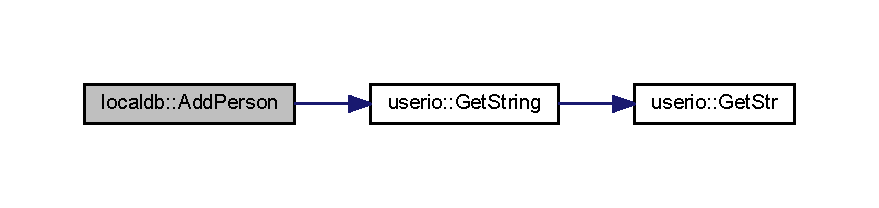
\includegraphics[width=350pt]{db/db5/classlocaldb_a4f24bb3dca226bf8e9dd3d923b82227b_cgraph}
\end{center}
\end{figure}




Here is the caller graph for this function\-:\nopagebreak
\begin{figure}[H]
\begin{center}
\leavevmode
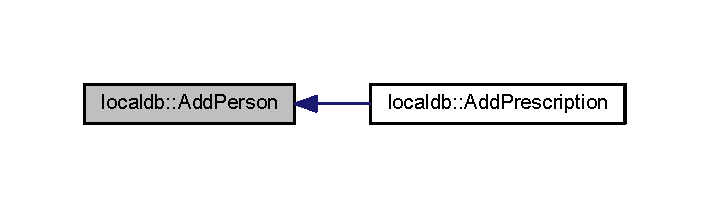
\includegraphics[width=340pt]{db/db5/classlocaldb_a4f24bb3dca226bf8e9dd3d923b82227b_icgraph}
\end{center}
\end{figure}


\hypertarget{classlocaldb_a90db632343f5cb21efce81507d5cff64}{\index{localdb@{localdb}!Add\-Prescription@{Add\-Prescription}}
\index{Add\-Prescription@{Add\-Prescription}!localdb@{localdb}}
\subsubsection[{Add\-Prescription}]{\setlength{\rightskip}{0pt plus 5cm}void localdb\-::\-Add\-Prescription (
\begin{DoxyParamCaption}
{}
\end{DoxyParamCaption}
)}}\label{db/db5/classlocaldb_a90db632343f5cb21efce81507d5cff64}
Requests information from the user to add a new prescription. Also adds new doctors / patients if these don't already exist. 

Here is the call graph for this function\-:\nopagebreak
\begin{figure}[H]
\begin{center}
\leavevmode
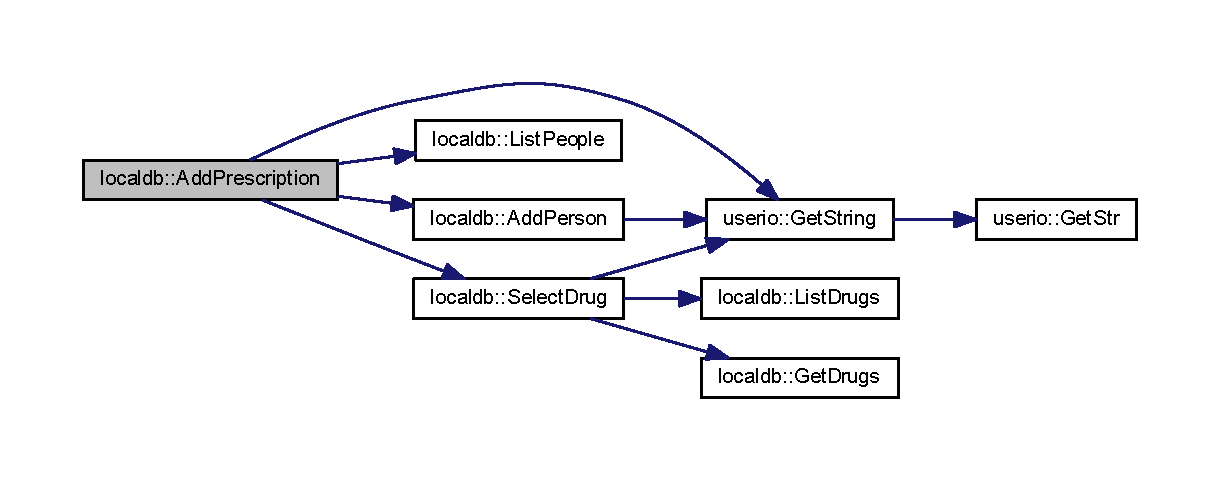
\includegraphics[width=350pt]{db/db5/classlocaldb_a90db632343f5cb21efce81507d5cff64_cgraph}
\end{center}
\end{figure}


\hypertarget{classlocaldb_a78cfa790e464e1868e11664c85fd2f71}{\index{localdb@{localdb}!Get\-Drugs@{Get\-Drugs}}
\index{Get\-Drugs@{Get\-Drugs}!localdb@{localdb}}
\subsubsection[{Get\-Drugs}]{\setlength{\rightskip}{0pt plus 5cm}Med\-List localdb\-::\-Get\-Drugs (
\begin{DoxyParamCaption}
\item[{const std\-::string}]{search, }
\item[{const int}]{search\-\_\-type}
\end{DoxyParamCaption}
)}}\label{db/db5/classlocaldb_a78cfa790e464e1868e11664c85fd2f71}
Searches rxnorm's medical database for the substance defined by the search parameter. Either by I\-D, name or estimated name match as defined by the search\-\_\-type parameter.


\begin{DoxyParams}{Parameters}
{\em const} & string search Contains the search string \\
\hline
{\em const} & integer search\-\_\-type How to search the A\-P\-I \\
\hline
\end{DoxyParams}
\begin{DoxyReturn}{Returns}
integer 
\end{DoxyReturn}


Here is the caller graph for this function\-:
\nopagebreak
\begin{figure}[H]
\begin{center}
\leavevmode
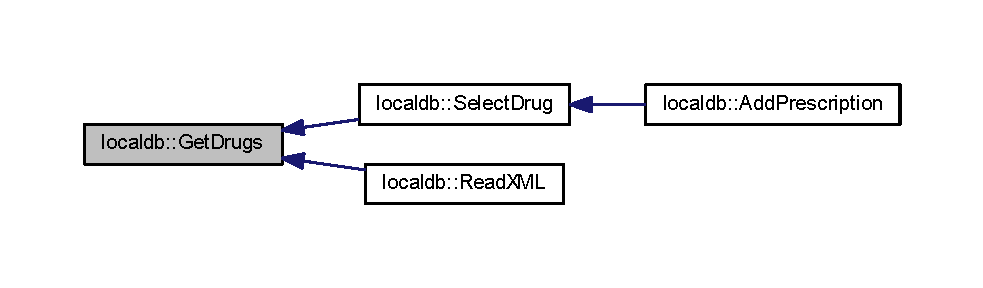
\includegraphics[width=350pt]{db/db5/classlocaldb_a78cfa790e464e1868e11664c85fd2f71_icgraph}
\end{center}
\end{figure}


\hypertarget{classlocaldb_ab99fbc1662afc289a14311d04cf70efe}{\index{localdb@{localdb}!Get\-Prescribed@{Get\-Prescribed}}
\index{Get\-Prescribed@{Get\-Prescribed}!localdb@{localdb}}
\subsubsection[{Get\-Prescribed}]{\setlength{\rightskip}{0pt plus 5cm}std\-::list$<$ {\bf prescription} $>$ localdb\-::\-Get\-Prescribed (
\begin{DoxyParamCaption}
\item[{std\-::string}]{search, }
\item[{int}]{how = {\ttfamily BY\-\_\-DRUG}}
\end{DoxyParamCaption}
)}}\label{db/db5/classlocaldb_ab99fbc1662afc289a14311d04cf70efe}
This method just routes the call depending on the 'how' parameter. i.\-e if how == B\-Y\-\_\-\-D\-R\-U\-G it will return the returnvalue for Get\-Prescription\-By\-Drug\-I\-D It then returns a list of prescriptions for that particular drug / doctor / patient


\begin{DoxyParams}{Parameters}
{\em string} & Search string (i.\-e doctors name, patient S\-S\-N, or drug I\-D) \\
\hline
{\em int} & how What criteria to find prescriptions for (B\-Y\-\_\-\-D\-R\-U\-G, B\-Y\-\_\-\-N\-A\-M\-E, B\-Y\-\_\-\-D\-O\-C\-T\-O\-R) \\
\hline
\end{DoxyParams}
\begin{DoxyReturn}{Returns}
list$<$prescription$>$ 
\end{DoxyReturn}
\hypertarget{classlocaldb_afb9a1b5b4ac821a205f4077b80c31c6a}{\index{localdb@{localdb}!List\-Drugs@{List\-Drugs}}
\index{List\-Drugs@{List\-Drugs}!localdb@{localdb}}
\subsubsection[{List\-Drugs}]{\setlength{\rightskip}{0pt plus 5cm}void localdb\-::\-List\-Drugs (
\begin{DoxyParamCaption}
{}
\end{DoxyParamCaption}
)}}\label{db/db5/classlocaldb_afb9a1b5b4ac821a205f4077b80c31c6a}
Lists all drugs in our medical list 

Here is the caller graph for this function\-:\nopagebreak
\begin{figure}[H]
\begin{center}
\leavevmode
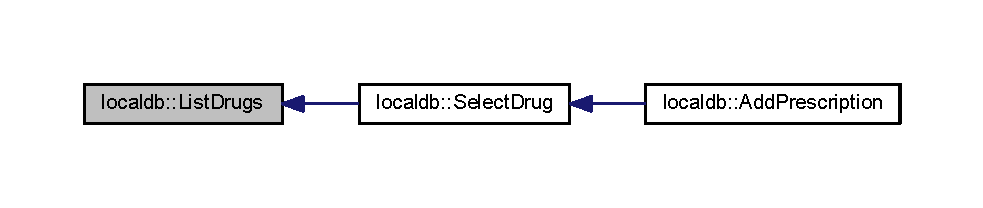
\includegraphics[width=350pt]{db/db5/classlocaldb_afb9a1b5b4ac821a205f4077b80c31c6a_icgraph}
\end{center}
\end{figure}


\hypertarget{classlocaldb_a4fd1d418a8acc517cf40f53ca9451840}{\index{localdb@{localdb}!List\-People@{List\-People}}
\index{List\-People@{List\-People}!localdb@{localdb}}
\subsubsection[{List\-People}]{\setlength{\rightskip}{0pt plus 5cm}void localdb\-::\-List\-People (
\begin{DoxyParamCaption}
\item[{int}]{type}
\end{DoxyParamCaption}
)}}\label{db/db5/classlocaldb_a4fd1d418a8acc517cf40f53ca9451840}
Lists all people of type (D\-O\-C\-T\-O\-R or P\-A\-T\-I\-E\-N\-T) Lists all people if no type is specified.


\begin{DoxyParams}{Parameters}
{\em int} & type Indicates if we're listing doctors or patients \\
\hline
\end{DoxyParams}


Here is the caller graph for this function\-:\nopagebreak
\begin{figure}[H]
\begin{center}
\leavevmode
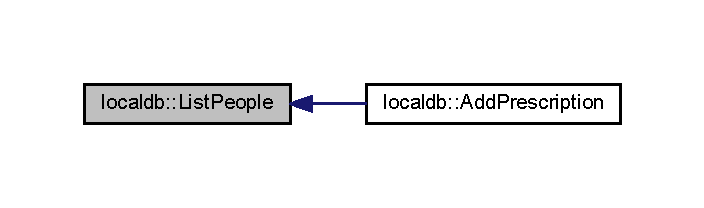
\includegraphics[width=338pt]{db/db5/classlocaldb_a4fd1d418a8acc517cf40f53ca9451840_icgraph}
\end{center}
\end{figure}


\hypertarget{classlocaldb_a03a61fd8105d78c2c91c852ac0f17c37}{\index{localdb@{localdb}!List\-Prescriptions@{List\-Prescriptions}}
\index{List\-Prescriptions@{List\-Prescriptions}!localdb@{localdb}}
\subsubsection[{List\-Prescriptions}]{\setlength{\rightskip}{0pt plus 5cm}void localdb\-::\-List\-Prescriptions (
\begin{DoxyParamCaption}
\item[{std\-::list$<$ {\bf prescription} $>$}]{pr}
\end{DoxyParamCaption}
)}}\label{db/db5/classlocaldb_a03a61fd8105d78c2c91c852ac0f17c37}
Lists all prescriptions in a prescriptionlist


\begin{DoxyParams}{Parameters}
{\em list$<$prescription$>$} & \\
\hline
\end{DoxyParams}
\hypertarget{classlocaldb_a21b2b2a127e94fd6a2124fe21271016e}{\index{localdb@{localdb}!Purge\-Old@{Purge\-Old}}
\index{Purge\-Old@{Purge\-Old}!localdb@{localdb}}
\subsubsection[{Purge\-Old}]{\setlength{\rightskip}{0pt plus 5cm}void localdb\-::\-Purge\-Old (
\begin{DoxyParamCaption}
\item[{time\-\_\-t}]{dt}
\end{DoxyParamCaption}
)}}\label{db/db5/classlocaldb_a21b2b2a127e94fd6a2124fe21271016e}
Purges old prescriptions


\begin{DoxyParams}{Parameters}
{\em time\-\_\-t} & dt Timestamp-\/limit -- anything older than this will be purged \\
\hline
\end{DoxyParams}
\hypertarget{classlocaldb_a5baa1e7864c62df9af7a0cba5b7ae517}{\index{localdb@{localdb}!Read\-X\-M\-L@{Read\-X\-M\-L}}
\index{Read\-X\-M\-L@{Read\-X\-M\-L}!localdb@{localdb}}
\subsubsection[{Read\-X\-M\-L}]{\setlength{\rightskip}{0pt plus 5cm}void localdb\-::\-Read\-X\-M\-L (
\begin{DoxyParamCaption}
{}
\end{DoxyParamCaption}
)}}\label{db/db5/classlocaldb_a5baa1e7864c62df9af7a0cba5b7ae517}
Reads the content of our local X\-M\-L database file and populates the Med\-Lists and People lists accordingly 

Here is the call graph for this function\-:
\nopagebreak
\begin{figure}[H]
\begin{center}
\leavevmode
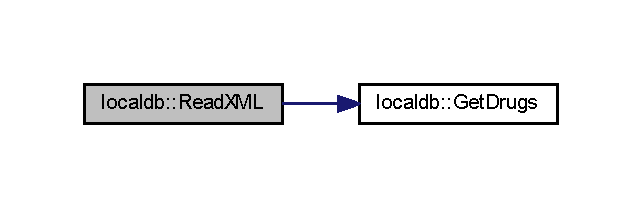
\includegraphics[width=308pt]{db/db5/classlocaldb_a5baa1e7864c62df9af7a0cba5b7ae517_cgraph}
\end{center}
\end{figure}


\hypertarget{classlocaldb_a1208a5ed6ca28d850d01bac6e09b673d}{\index{localdb@{localdb}!Select\-Drug@{Select\-Drug}}
\index{Select\-Drug@{Select\-Drug}!localdb@{localdb}}
\subsubsection[{Select\-Drug}]{\setlength{\rightskip}{0pt plus 5cm}{\bf medicine} localdb\-::\-Select\-Drug (
\begin{DoxyParamCaption}
{}
\end{DoxyParamCaption}
)}}\label{db/db5/classlocaldb_a1208a5ed6ca28d850d01bac6e09b673d}
Lets the user select a drug by entering the drug I\-D The drug I\-D can be found online (as provided to the user should he enter 'search') or locally, if a previous prescription has been made for that drug (as provided to the user should he enter 'list'). Returns the selected drug as a medicine struct

\begin{DoxyReturn}{Returns}
medicine 
\end{DoxyReturn}


Here is the call graph for this function\-:\nopagebreak
\begin{figure}[H]
\begin{center}
\leavevmode
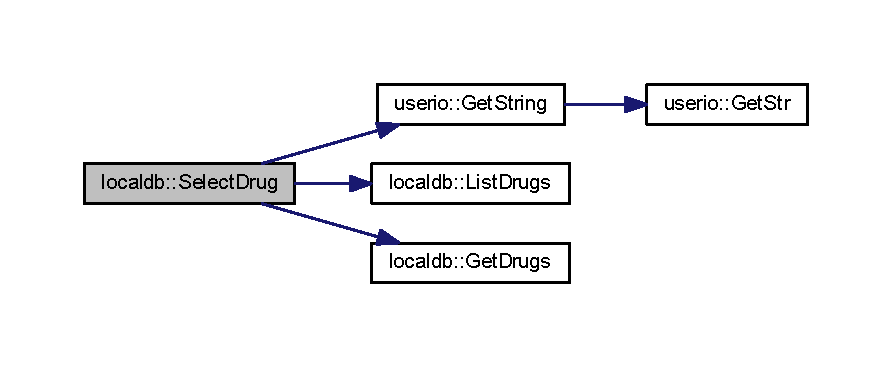
\includegraphics[width=350pt]{db/db5/classlocaldb_a1208a5ed6ca28d850d01bac6e09b673d_cgraph}
\end{center}
\end{figure}




Here is the caller graph for this function\-:\nopagebreak
\begin{figure}[H]
\begin{center}
\leavevmode
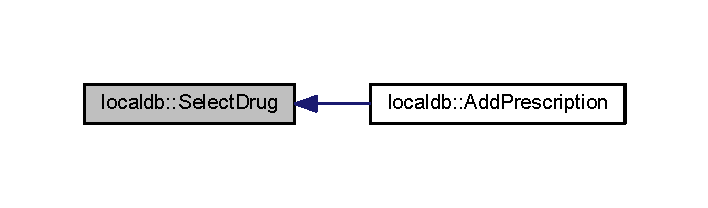
\includegraphics[width=340pt]{db/db5/classlocaldb_a1208a5ed6ca28d850d01bac6e09b673d_icgraph}
\end{center}
\end{figure}


\hypertarget{classlocaldb_a81660b43bd6e610c770ff3bcf5e4c72a}{\index{localdb@{localdb}!Write\-X\-M\-L@{Write\-X\-M\-L}}
\index{Write\-X\-M\-L@{Write\-X\-M\-L}!localdb@{localdb}}
\subsubsection[{Write\-X\-M\-L}]{\setlength{\rightskip}{0pt plus 5cm}void localdb\-::\-Write\-X\-M\-L (
\begin{DoxyParamCaption}
{}
\end{DoxyParamCaption}
)}}\label{db/db5/classlocaldb_a81660b43bd6e610c770ff3bcf5e4c72a}
Outputs all stored data to local X\-M\-L database file Pretty much the same as the \hyperlink{classlocaldb_a5baa1e7864c62df9af7a0cba5b7ae517}{Read\-X\-M\-L()} method, but reversed 

The documentation for this class was generated from the following files\-:\begin{DoxyCompactItemize}
\item 
localdb.\-h\item 
localdb.\-cpp\end{DoxyCompactItemize}

\hypertarget{structmedicine}{\section{medicine Struct Reference}
\label{d3/d07/structmedicine}\index{medicine@{medicine}}
}
\subsection*{Public Attributes}
\begin{DoxyCompactItemize}
\item 
\hypertarget{structmedicine_acd4f4546c02656c5849c7f39f7660acc}{std\-::string {\bfseries name}}\label{d3/d07/structmedicine_acd4f4546c02656c5849c7f39f7660acc}

\item 
\hypertarget{structmedicine_ade31a1a6210f4f7e2b37832a35593c0c}{std\-::string {\bfseries market\-\_\-name}}\label{d3/d07/structmedicine_ade31a1a6210f4f7e2b37832a35593c0c}

\item 
\hypertarget{structmedicine_a503c1beb4a3c6fa53cc59b565f447e20}{std\-::string {\bfseries rxnorm\-\_\-id}}\label{d3/d07/structmedicine_a503c1beb4a3c6fa53cc59b565f447e20}

\item 
\hypertarget{structmedicine_a5b32c9cab1b2ae4406a46f3dd5f152b8}{std\-::string {\bfseries concept\-\_\-id}}\label{d3/d07/structmedicine_a5b32c9cab1b2ae4406a46f3dd5f152b8}

\item 
\hypertarget{structmedicine_ac9f661459d431ae0eadf430fa00f941d}{std\-::string {\bfseries strength}}\label{d3/d07/structmedicine_ac9f661459d431ae0eadf430fa00f941d}

\item 
\hypertarget{structmedicine_a7241be98632597337542dba7c772687c}{std\-::string {\bfseries quantity}}\label{d3/d07/structmedicine_a7241be98632597337542dba7c772687c}

\end{DoxyCompactItemize}


The documentation for this struct was generated from the following file\-:\begin{DoxyCompactItemize}
\item 
prescription.\-h\end{DoxyCompactItemize}

\hypertarget{class_num__element}{\section{Num\-\_\-element Class Reference}
\label{d8/d1c/class_num__element}\index{Num\-\_\-element@{Num\-\_\-element}}
}


Inheritance diagram for Num\-\_\-element\-:\nopagebreak
\begin{figure}[H]
\begin{center}
\leavevmode
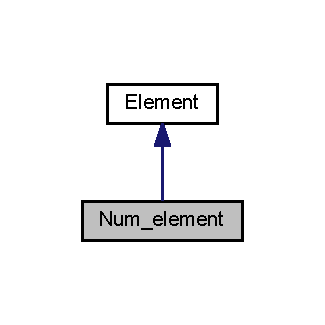
\includegraphics[width=156pt]{d0/daf/class_num__element__inherit__graph}
\end{center}
\end{figure}


Collaboration diagram for Num\-\_\-element\-:\nopagebreak
\begin{figure}[H]
\begin{center}
\leavevmode
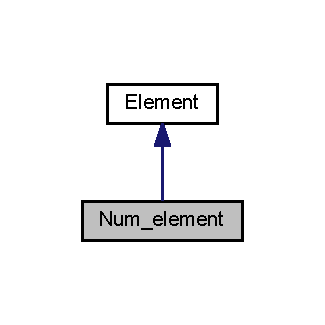
\includegraphics[width=156pt]{d7/d29/class_num__element__coll__graph}
\end{center}
\end{figure}
\subsection*{Public Member Functions}
\begin{DoxyCompactItemize}
\item 
\hypertarget{class_num__element_ad99dd33f81ad3fe59c219bee2bbbb951}{{\bfseries Num\-\_\-element} (int no)}\label{d8/d1c/class_num__element_ad99dd33f81ad3fe59c219bee2bbbb951}

\item 
\hypertarget{class_num__element_ac4a144cd601fc276efb1b3141ddcee65}{virtual int {\bfseries compare} (\hyperlink{class_element}{Element} $\ast$el)}\label{d8/d1c/class_num__element_ac4a144cd601fc276efb1b3141ddcee65}

\end{DoxyCompactItemize}
\subsection*{Protected Attributes}
\begin{DoxyCompactItemize}
\item 
\hypertarget{class_num__element_a2a4b3a4fc6592ddc625786804e4800f2}{int {\bfseries number}}\label{d8/d1c/class_num__element_a2a4b3a4fc6592ddc625786804e4800f2}

\end{DoxyCompactItemize}


The documentation for this class was generated from the following files\-:\begin{DoxyCompactItemize}
\item 
list\-\_\-tool.\-h\item 
list\-\_\-tool.\-cpp\end{DoxyCompactItemize}

\hypertarget{classperson}{\section{person Class Reference}
\label{d7/db3/classperson}\index{person@{person}}
}
\subsection*{Public Member Functions}
\begin{DoxyCompactItemize}
\item 
\hypertarget{classperson_ae51e4db2f4062727dafa2360235a1af0}{std\-::string {\bfseries Get\-First\-Name} ()}\label{d7/db3/classperson_ae51e4db2f4062727dafa2360235a1af0}

\item 
\hypertarget{classperson_a4071fb0ed9c89dbdc28edbec0169d8a4}{std\-::string {\bfseries Get\-Last\-Name} ()}\label{d7/db3/classperson_a4071fb0ed9c89dbdc28edbec0169d8a4}

\item 
\hypertarget{classperson_a89f2b1d68585cf75f42342a16f90f807}{std\-::string {\bfseries Get\-Address} ()}\label{d7/db3/classperson_a89f2b1d68585cf75f42342a16f90f807}

\item 
\hypertarget{classperson_a31df9be3d36abb32526b5058f6053a21}{std\-::string {\bfseries Get\-S\-S\-N} ()}\label{d7/db3/classperson_a31df9be3d36abb32526b5058f6053a21}

\item 
\hypertarget{classperson_a51e27cd24d7767277a28c27c7b933eeb}{std\-::string {\bfseries Get\-Zip} ()}\label{d7/db3/classperson_a51e27cd24d7767277a28c27c7b933eeb}

\item 
\hypertarget{classperson_a2ba50f2ea2725ac0819f245426bec37f}{std\-::string {\bfseries Get\-Phone} ()}\label{d7/db3/classperson_a2ba50f2ea2725ac0819f245426bec37f}

\item 
\hypertarget{classperson_a95073ba3711f5152accbc1e055ebcd92}{void {\bfseries Set\-First\-Name} (std\-::string val)}\label{d7/db3/classperson_a95073ba3711f5152accbc1e055ebcd92}

\item 
\hypertarget{classperson_af4a18f7bd8fc7d4a480b47332634d2c4}{void {\bfseries Set\-Last\-Name} (std\-::string val)}\label{d7/db3/classperson_af4a18f7bd8fc7d4a480b47332634d2c4}

\item 
\hypertarget{classperson_a8b9a2ba042f86f3fe1c20c900c3585ac}{void {\bfseries Set\-Address} (std\-::string val)}\label{d7/db3/classperson_a8b9a2ba042f86f3fe1c20c900c3585ac}

\item 
\hypertarget{classperson_add13137925787bacf3b41e1f441d1229}{void {\bfseries Set\-S\-S\-N} (std\-::string val)}\label{d7/db3/classperson_add13137925787bacf3b41e1f441d1229}

\item 
\hypertarget{classperson_a5456f5de42df1b8cfae23b6325caacf6}{void {\bfseries Set\-Zip} (std\-::string val)}\label{d7/db3/classperson_a5456f5de42df1b8cfae23b6325caacf6}

\item 
\hypertarget{classperson_aadbd4c38d5f1f6f49b91ebe816c16575}{void {\bfseries Set\-Phone} (std\-::string val)}\label{d7/db3/classperson_aadbd4c38d5f1f6f49b91ebe816c16575}

\end{DoxyCompactItemize}


The documentation for this class was generated from the following files\-:\begin{DoxyCompactItemize}
\item 
person.\-h\item 
person.\-cpp\end{DoxyCompactItemize}

\hypertarget{classprescription}{\section{prescription Class Reference}
\label{d0/dd9/classprescription}\index{prescription@{prescription}}
}
\subsection*{Public Member Functions}
\begin{DoxyCompactItemize}
\item 
\hypertarget{classprescription_a03733b36abadb1d5cb04e126a79d3237}{{\bfseries prescription} (struct tm date)}\label{d0/dd9/classprescription_a03733b36abadb1d5cb04e126a79d3237}

\item 
\hypertarget{classprescription_a863f80f57af060d86ed8f089c3779afb}{{\bfseries prescription} (\hyperlink{classperson}{person} $\ast$dr, \hyperlink{classperson}{person} $\ast$ptnt, time\-\_\-t dt=time(N\-U\-L\-L))}\label{d0/dd9/classprescription_a863f80f57af060d86ed8f089c3779afb}

\item 
\hypertarget{classprescription_af1f7834158a21749b9a8f4c3e975aa4b}{{\bfseries prescription} (\hyperlink{classperson}{person} $\ast$dr, \hyperlink{classperson}{person} $\ast$ptnt, \hyperlink{structmedicine}{medicine} $\ast$drg, time\-\_\-t dt=time(N\-U\-L\-L))}\label{d0/dd9/classprescription_af1f7834158a21749b9a8f4c3e975aa4b}

\item 
\hypertarget{classprescription_afb30c7295fd7fa2627ff622d1fc176b9}{time\-\_\-t {\bfseries Get\-Date} ()}\label{d0/dd9/classprescription_afb30c7295fd7fa2627ff622d1fc176b9}

\item 
\hypertarget{classprescription_ae1240cbb14197dd98f71367b71dc98c4}{std\-::string {\bfseries Get\-Dosage} ()}\label{d0/dd9/classprescription_ae1240cbb14197dd98f71367b71dc98c4}

\item 
\hypertarget{classprescription_abada4fa8c7787b2144903de430033679}{\hyperlink{classperson}{person} \& {\bfseries Get\-Doctor} ()}\label{d0/dd9/classprescription_abada4fa8c7787b2144903de430033679}

\item 
\hypertarget{classprescription_a1e72c9b1f889eb61a63c1689053e878e}{\hyperlink{classperson}{person} \& {\bfseries Get\-Patient} ()}\label{d0/dd9/classprescription_a1e72c9b1f889eb61a63c1689053e878e}

\item 
\hypertarget{classprescription_ab0db387bdcc5b44e29a72c862d24426b}{\hyperlink{structmedicine}{medicine} $\ast$ {\bfseries Get\-Drug} ()}\label{d0/dd9/classprescription_ab0db387bdcc5b44e29a72c862d24426b}

\item 
void \hyperlink{classprescription_a1e876ae983decf3c3e4425dfccd64805}{Set\-Hour} (int h)
\item 
void \hyperlink{classprescription_a35c70e5bcdf1263afd2a52f6e47accbd}{Set\-Minute} (int m)
\item 
void \hyperlink{classprescription_a5efb71a441fa5671a60180ca30b5882b}{Set\-Second} (int s)
\item 
void \hyperlink{classprescription_a093553b6c876eefd7933864ddf6fef97}{Set\-Day} (int d)
\item 
void \hyperlink{classprescription_a8272667bc6cecf8b242362ca1ae801c3}{Set\-Month} (int m)
\item 
void \hyperlink{classprescription_a76114a03aea0bb0d56084268d5d89608}{Set\-Year} (int y)
\item 
void \hyperlink{classprescription_aa5272268cd360a4376ff2a8c05d8d240}{Set\-Date} (time\-\_\-t d)
\item 
void \hyperlink{classprescription_a9e19ba585000fe3d662f4c59102806c7}{Set\-Time} (time\-\_\-t date=time(N\-U\-L\-L))
\item 
\hypertarget{classprescription_a298a366067d002733400cfdee817bced}{void {\bfseries Set\-Drug} (\hyperlink{structmedicine}{medicine} $\ast$med)}\label{d0/dd9/classprescription_a298a366067d002733400cfdee817bced}

\item 
\hypertarget{classprescription_a70d211d36d42f8f1379aaed0b09466c3}{void {\bfseries Set\-Doctor} (\hyperlink{classperson}{person} $\ast$dr)}\label{d0/dd9/classprescription_a70d211d36d42f8f1379aaed0b09466c3}

\item 
\hypertarget{classprescription_a051c3d3aed8aefaf6ba8b48869842011}{void {\bfseries Set\-Patient} (\hyperlink{classperson}{person} $\ast$ptnt)}\label{d0/dd9/classprescription_a051c3d3aed8aefaf6ba8b48869842011}

\end{DoxyCompactItemize}


\subsection{Member Function Documentation}
\hypertarget{classprescription_aa5272268cd360a4376ff2a8c05d8d240}{\index{prescription@{prescription}!Set\-Date@{Set\-Date}}
\index{Set\-Date@{Set\-Date}!prescription@{prescription}}
\subsubsection[{Set\-Date}]{\setlength{\rightskip}{0pt plus 5cm}void prescription\-::\-Set\-Date (
\begin{DoxyParamCaption}
\item[{time\-\_\-t}]{d}
\end{DoxyParamCaption}
)}}\label{d0/dd9/classprescription_aa5272268cd360a4376ff2a8c05d8d240}
Sets the timestamp manually


\begin{DoxyParams}{Parameters}
{\em integer} & d Timestamp \\
\hline
\end{DoxyParams}


Here is the caller graph for this function\-:\nopagebreak
\begin{figure}[H]
\begin{center}
\leavevmode
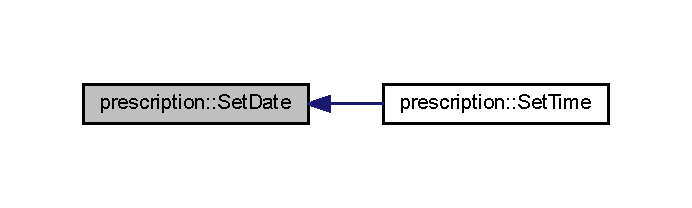
\includegraphics[width=332pt]{d0/dd9/classprescription_aa5272268cd360a4376ff2a8c05d8d240_icgraph}
\end{center}
\end{figure}


\hypertarget{classprescription_a093553b6c876eefd7933864ddf6fef97}{\index{prescription@{prescription}!Set\-Day@{Set\-Day}}
\index{Set\-Day@{Set\-Day}!prescription@{prescription}}
\subsubsection[{Set\-Day}]{\setlength{\rightskip}{0pt plus 5cm}void prescription\-::\-Set\-Day (
\begin{DoxyParamCaption}
\item[{int}]{d}
\end{DoxyParamCaption}
)}}\label{d0/dd9/classprescription_a093553b6c876eefd7933864ddf6fef97}
Sets the day specified by integer parameter d


\begin{DoxyParams}{Parameters}
{\em integer} & d Day of the month to set time to \\
\hline
\end{DoxyParams}
\hypertarget{classprescription_a1e876ae983decf3c3e4425dfccd64805}{\index{prescription@{prescription}!Set\-Hour@{Set\-Hour}}
\index{Set\-Hour@{Set\-Hour}!prescription@{prescription}}
\subsubsection[{Set\-Hour}]{\setlength{\rightskip}{0pt plus 5cm}void prescription\-::\-Set\-Hour (
\begin{DoxyParamCaption}
\item[{int}]{h}
\end{DoxyParamCaption}
)}}\label{d0/dd9/classprescription_a1e876ae983decf3c3e4425dfccd64805}
Sets the hour specified by integer parameter h


\begin{DoxyParams}{Parameters}
{\em integer} & h Hour to set time to \\
\hline
\end{DoxyParams}
\hypertarget{classprescription_a35c70e5bcdf1263afd2a52f6e47accbd}{\index{prescription@{prescription}!Set\-Minute@{Set\-Minute}}
\index{Set\-Minute@{Set\-Minute}!prescription@{prescription}}
\subsubsection[{Set\-Minute}]{\setlength{\rightskip}{0pt plus 5cm}void prescription\-::\-Set\-Minute (
\begin{DoxyParamCaption}
\item[{int}]{m}
\end{DoxyParamCaption}
)}}\label{d0/dd9/classprescription_a35c70e5bcdf1263afd2a52f6e47accbd}
Sets the minute specified by integer parameter m


\begin{DoxyParams}{Parameters}
{\em integer} & m Minute to set time to \\
\hline
\end{DoxyParams}
\hypertarget{classprescription_a8272667bc6cecf8b242362ca1ae801c3}{\index{prescription@{prescription}!Set\-Month@{Set\-Month}}
\index{Set\-Month@{Set\-Month}!prescription@{prescription}}
\subsubsection[{Set\-Month}]{\setlength{\rightskip}{0pt plus 5cm}void prescription\-::\-Set\-Month (
\begin{DoxyParamCaption}
\item[{int}]{m}
\end{DoxyParamCaption}
)}}\label{d0/dd9/classprescription_a8272667bc6cecf8b242362ca1ae801c3}
Sets the month specified by integer parameter m


\begin{DoxyParams}{Parameters}
{\em integer} & m Month to set time to \\
\hline
\end{DoxyParams}
\hypertarget{classprescription_a5efb71a441fa5671a60180ca30b5882b}{\index{prescription@{prescription}!Set\-Second@{Set\-Second}}
\index{Set\-Second@{Set\-Second}!prescription@{prescription}}
\subsubsection[{Set\-Second}]{\setlength{\rightskip}{0pt plus 5cm}void prescription\-::\-Set\-Second (
\begin{DoxyParamCaption}
\item[{int}]{s}
\end{DoxyParamCaption}
)}}\label{d0/dd9/classprescription_a5efb71a441fa5671a60180ca30b5882b}
Sets the second specified by integer parameter s


\begin{DoxyParams}{Parameters}
{\em integer} & s Second to set time to \\
\hline
\end{DoxyParams}
\hypertarget{classprescription_a9e19ba585000fe3d662f4c59102806c7}{\index{prescription@{prescription}!Set\-Time@{Set\-Time}}
\index{Set\-Time@{Set\-Time}!prescription@{prescription}}
\subsubsection[{Set\-Time}]{\setlength{\rightskip}{0pt plus 5cm}void prescription\-::\-Set\-Time (
\begin{DoxyParamCaption}
\item[{time\-\_\-t}]{d = {\ttfamily time(NULL)}}
\end{DoxyParamCaption}
)}}\label{d0/dd9/classprescription_a9e19ba585000fe3d662f4c59102806c7}
Sets the timestamp manually (A\-N\-D updates tmp\-Date accordingly)


\begin{DoxyParams}{Parameters}
{\em integer} & d Timestamp \\
\hline
\end{DoxyParams}


Here is the call graph for this function\-:\nopagebreak
\begin{figure}[H]
\begin{center}
\leavevmode
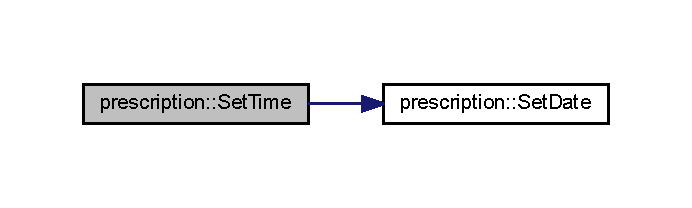
\includegraphics[width=332pt]{d0/dd9/classprescription_a9e19ba585000fe3d662f4c59102806c7_cgraph}
\end{center}
\end{figure}


\hypertarget{classprescription_a76114a03aea0bb0d56084268d5d89608}{\index{prescription@{prescription}!Set\-Year@{Set\-Year}}
\index{Set\-Year@{Set\-Year}!prescription@{prescription}}
\subsubsection[{Set\-Year}]{\setlength{\rightskip}{0pt plus 5cm}void prescription\-::\-Set\-Year (
\begin{DoxyParamCaption}
\item[{int}]{y}
\end{DoxyParamCaption}
)}}\label{d0/dd9/classprescription_a76114a03aea0bb0d56084268d5d89608}
Sets the year specified by integer parameter y


\begin{DoxyParams}{Parameters}
{\em integer} & y Year to set time to \\
\hline
\end{DoxyParams}


The documentation for this class was generated from the following files\-:\begin{DoxyCompactItemize}
\item 
prescription.\-h\item 
prescription.\-cpp\end{DoxyCompactItemize}

\hypertarget{classsubstance}{\section{substance Class Reference}
\label{d3/df8/classsubstance}\index{substance@{substance}}
}


The documentation for this class was generated from the following files\-:\begin{DoxyCompactItemize}
\item 
substance.\-h\item 
substance.\-cpp\end{DoxyCompactItemize}

\hypertarget{class_text__element}{\section{Text\-\_\-element Class Reference}
\label{db/d3d/class_text__element}\index{Text\-\_\-element@{Text\-\_\-element}}
}


Inheritance diagram for Text\-\_\-element\-:\nopagebreak
\begin{figure}[H]
\begin{center}
\leavevmode
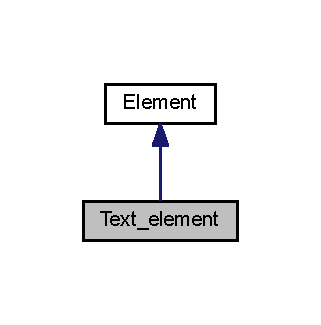
\includegraphics[width=154pt]{d8/d25/class_text__element__inherit__graph}
\end{center}
\end{figure}


Collaboration diagram for Text\-\_\-element\-:\nopagebreak
\begin{figure}[H]
\begin{center}
\leavevmode
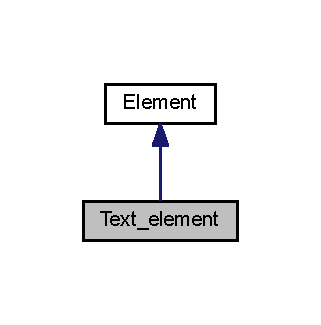
\includegraphics[width=154pt]{db/d7d/class_text__element__coll__graph}
\end{center}
\end{figure}
\subsection*{Public Member Functions}
\begin{DoxyCompactItemize}
\item 
\hypertarget{class_text__element_a3c2586285468c3fede70e5a4812c8517}{{\bfseries Text\-\_\-element} (const char $\ast$t)}\label{db/d3d/class_text__element_a3c2586285468c3fede70e5a4812c8517}

\item 
\hypertarget{class_text__element_a9794e999b859accdceda478c74b2c156}{virtual int {\bfseries compare} (\hyperlink{class_element}{Element} $\ast$el)}\label{db/d3d/class_text__element_a9794e999b859accdceda478c74b2c156}

\end{DoxyCompactItemize}
\subsection*{Protected Attributes}
\begin{DoxyCompactItemize}
\item 
\hypertarget{class_text__element_aa88cdc32a5a73e36d782ee63580662e6}{char $\ast$ {\bfseries text}}\label{db/d3d/class_text__element_aa88cdc32a5a73e36d782ee63580662e6}

\end{DoxyCompactItemize}


The documentation for this class was generated from the following files\-:\begin{DoxyCompactItemize}
\item 
list\-\_\-tool.\-h\item 
list\-\_\-tool.\-cpp\end{DoxyCompactItemize}

\hypertarget{classuserio}{\section{userio Class Reference}
\label{dc/ddf/classuserio}\index{userio@{userio}}
}
\subsection*{Public Types}
\begin{DoxyCompactItemize}
\item 
enum \{ \\*
{\bfseries N\-O\-F\-I\-L\-T\-E\-R}, 
{\bfseries M\-I\-N}, 
{\bfseries M\-A\-X}, 
{\bfseries B\-E\-T\-W\-E\-E\-N}, 
\\*
{\bfseries E\-Q\-U\-A\-L\-S}, 
{\bfseries N\-O\-T}, 
{\bfseries C\-O\-N\-T\-A\-I\-N\-S}
 \}
\end{DoxyCompactItemize}
\subsection*{Static Public Member Functions}
\begin{DoxyCompactItemize}
\item 
static char \hyperlink{classuserio_a4b9f8afe7fb2bd76f5266a684cd20d04}{Get\-Char} (std\-::string pre, int how, char alt1= '-\/', char alt2= '-\/')
\item 
static int \hyperlink{classuserio_a1c7d7816b8685f249f6cdb9daf524730}{Get\-Int} (std\-::string pre, int how, int alt1, int alt2=0)
\item 
static std\-::string \hyperlink{classuserio_ae31f1f0b7982933a8c9ac5ac683b7450}{Get\-String} (std\-::string pre, int how, std\-::string str1=\char`\"{}\char`\"{}, const int min=0, unsigned const int max=0)
\item 
static std\-::string \hyperlink{classuserio_a8cce5c74bcb42130d51d28dca9cca56c}{Get\-String} (std\-::string pre, std\-::string regex, std\-::string readable\-\_\-regex)
\item 
static time\-\_\-t \hyperlink{classuserio_ad764988b25a5491ff4d09f096aaa3e36}{Get\-Timestamp} (std\-::string pre)
\item 
static struct tm \hyperlink{classuserio_ad89aefb694383c172e04af7efb2a96fa}{Get\-Time} (std\-::string pre)
\item 
static struct tm \hyperlink{classuserio_a29176550beb6b7abf9d9a6093a2fc484}{Get\-Date} (std\-::string pre)
\item 
static time\-\_\-t \hyperlink{classuserio_a815f7bcecc23024e5b2e7a2584f13222}{Make\-Timestamp} (struct tm clock, struct tm date)
\item 
static char \hyperlink{classuserio_a9628539a58d68f72ca969d4e56a20fd7}{Get\-Char} ()
\item 
static int \hyperlink{classuserio_aa27b9bea4db93f6c323bd3124e6cebb2}{Get\-Num} ()
\item 
\hypertarget{classuserio_a53cc662c35b86ddc0ceb3b3f490621bb}{static char $\ast$ {\bfseries Getp\-Char} ()}\label{dc/ddf/classuserio_a53cc662c35b86ddc0ceb3b3f490621bb}

\item 
static std\-::string \hyperlink{classuserio_a4bcb13a6da031a044765003a310b9df5}{Get\-Str} ()
\end{DoxyCompactItemize}


\subsection{Member Function Documentation}
\hypertarget{classuserio_a4b9f8afe7fb2bd76f5266a684cd20d04}{\index{userio@{userio}!Get\-Char@{Get\-Char}}
\index{Get\-Char@{Get\-Char}!userio@{userio}}
\subsubsection[{Get\-Char}]{\setlength{\rightskip}{0pt plus 5cm}char userio\-::\-Get\-Char (
\begin{DoxyParamCaption}
\item[{std\-::string}]{pre, }
\item[{int}]{how, }
\item[{char}]{alt1 = {\ttfamily '-\/'}, }
\item[{char}]{alt2 = {\ttfamily '-\/'}}
\end{DoxyParamCaption}
)\hspace{0.3cm}{\ttfamily [static]}}}\label{dc/ddf/classuserio_a4b9f8afe7fb2bd76f5266a684cd20d04}
Sanitizes a char (as determined by the interaction enum 'how')


\begin{DoxyParams}{Parameters}
{\em string} & pre Text to print before catching users input \\
\hline
{\em integer} & how Determines how the expected char should be \\
\hline
{\em char} & alt1 Used when 'how' is E\-Q\-U\-A\-L\-S, B\-E\-T\-W\-E\-E\-N, N\-O\-T, or C\-O\-N\-T\-A\-I\-N\-S to compare against \\
\hline
{\em char} & alt2 Used when 'how' is E\-Q\-U\-A\-L\-S or B\-E\-T\-W\-E\-E\-N in conjunction with alt1 \\
\hline
\end{DoxyParams}
\begin{DoxyReturn}{Returns}
char 
\end{DoxyReturn}


Here is the call graph for this function\-:\nopagebreak
\begin{figure}[H]
\begin{center}
\leavevmode
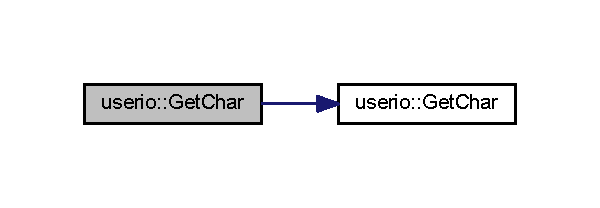
\includegraphics[width=288pt]{dc/ddf/classuserio_a4b9f8afe7fb2bd76f5266a684cd20d04_cgraph}
\end{center}
\end{figure}


\hypertarget{classuserio_a9628539a58d68f72ca969d4e56a20fd7}{\index{userio@{userio}!Get\-Char@{Get\-Char}}
\index{Get\-Char@{Get\-Char}!userio@{userio}}
\subsubsection[{Get\-Char}]{\setlength{\rightskip}{0pt plus 5cm}char userio\-::\-Get\-Char (
\begin{DoxyParamCaption}
{}
\end{DoxyParamCaption}
)\hspace{0.3cm}{\ttfamily [static]}}}\label{dc/ddf/classuserio_a9628539a58d68f72ca969d4e56a20fd7}
Gets a char from the user through the input stream

\begin{DoxyReturn}{Returns}
char 
\end{DoxyReturn}


Here is the caller graph for this function\-:\nopagebreak
\begin{figure}[H]
\begin{center}
\leavevmode
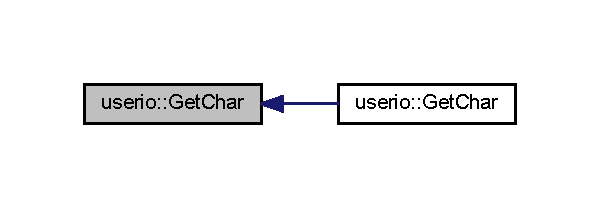
\includegraphics[width=288pt]{dc/ddf/classuserio_a9628539a58d68f72ca969d4e56a20fd7_icgraph}
\end{center}
\end{figure}


\hypertarget{classuserio_a29176550beb6b7abf9d9a6093a2fc484}{\index{userio@{userio}!Get\-Date@{Get\-Date}}
\index{Get\-Date@{Get\-Date}!userio@{userio}}
\subsubsection[{Get\-Date}]{\setlength{\rightskip}{0pt plus 5cm}struct tm userio\-::\-Get\-Date (
\begin{DoxyParamCaption}
\item[{std\-::string}]{pre}
\end{DoxyParamCaption}
)\hspace{0.3cm}{\ttfamily [static]}, {\ttfamily [read]}}}\label{dc/ddf/classuserio_a29176550beb6b7abf9d9a6093a2fc484}
Creates a timestruct from userprovided date.


\begin{DoxyParams}{Parameters}
{\em string} & pre Pretext to show before taking input \\
\hline
\end{DoxyParams}
\begin{DoxyReturn}{Returns}
struct tm 
\end{DoxyReturn}


Here is the caller graph for this function\-:\nopagebreak
\begin{figure}[H]
\begin{center}
\leavevmode
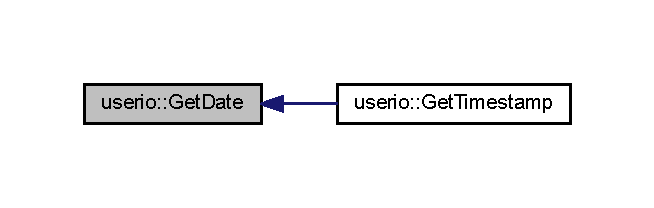
\includegraphics[width=314pt]{dc/ddf/classuserio_a29176550beb6b7abf9d9a6093a2fc484_icgraph}
\end{center}
\end{figure}


\hypertarget{classuserio_a1c7d7816b8685f249f6cdb9daf524730}{\index{userio@{userio}!Get\-Int@{Get\-Int}}
\index{Get\-Int@{Get\-Int}!userio@{userio}}
\subsubsection[{Get\-Int}]{\setlength{\rightskip}{0pt plus 5cm}int userio\-::\-Get\-Int (
\begin{DoxyParamCaption}
\item[{std\-::string}]{pre, }
\item[{int}]{how, }
\item[{int}]{alt1, }
\item[{int}]{alt2 = {\ttfamily 0}}
\end{DoxyParamCaption}
)\hspace{0.3cm}{\ttfamily [static]}}}\label{dc/ddf/classuserio_a1c7d7816b8685f249f6cdb9daf524730}
Sanitizes an integer (as determined by the interaction enum 'how')


\begin{DoxyParams}{Parameters}
{\em string} & pre Text to print before catching users input \\
\hline
{\em integer} & how Determines how the expected integer should be \\
\hline
{\em int} & alt1 Used when 'how' is E\-Q\-U\-A\-L\-S, B\-E\-T\-W\-E\-E\-N, N\-O\-T, or C\-O\-N\-T\-A\-I\-N\-S to compare against \\
\hline
{\em int} & alt2 Used when 'how' is E\-Q\-U\-A\-L\-S, B\-E\-T\-W\-E\-E\-N or N\-O\-T in conjunction with alt1 \\
\hline
\end{DoxyParams}
\begin{DoxyReturn}{Returns}
int 
\end{DoxyReturn}


Here is the call graph for this function\-:\nopagebreak
\begin{figure}[H]
\begin{center}
\leavevmode
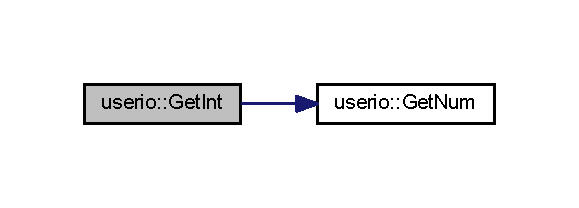
\includegraphics[width=278pt]{dc/ddf/classuserio_a1c7d7816b8685f249f6cdb9daf524730_cgraph}
\end{center}
\end{figure}


\hypertarget{classuserio_aa27b9bea4db93f6c323bd3124e6cebb2}{\index{userio@{userio}!Get\-Num@{Get\-Num}}
\index{Get\-Num@{Get\-Num}!userio@{userio}}
\subsubsection[{Get\-Num}]{\setlength{\rightskip}{0pt plus 5cm}int userio\-::\-Get\-Num (
\begin{DoxyParamCaption}
{}
\end{DoxyParamCaption}
)\hspace{0.3cm}{\ttfamily [static]}}}\label{dc/ddf/classuserio_aa27b9bea4db93f6c323bd3124e6cebb2}
Gets an integer from the user through the input stream

\begin{DoxyReturn}{Returns}
integer 
\end{DoxyReturn}


Here is the caller graph for this function\-:\nopagebreak
\begin{figure}[H]
\begin{center}
\leavevmode
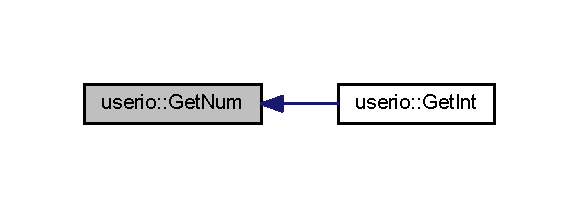
\includegraphics[width=278pt]{dc/ddf/classuserio_aa27b9bea4db93f6c323bd3124e6cebb2_icgraph}
\end{center}
\end{figure}


\hypertarget{classuserio_a4bcb13a6da031a044765003a310b9df5}{\index{userio@{userio}!Get\-Str@{Get\-Str}}
\index{Get\-Str@{Get\-Str}!userio@{userio}}
\subsubsection[{Get\-Str}]{\setlength{\rightskip}{0pt plus 5cm}std\-::string userio\-::\-Get\-Str (
\begin{DoxyParamCaption}
{}
\end{DoxyParamCaption}
)\hspace{0.3cm}{\ttfamily [static]}}}\label{dc/ddf/classuserio_a4bcb13a6da031a044765003a310b9df5}
Gets a string from the user through the input stream

\begin{DoxyReturn}{Returns}
string 
\end{DoxyReturn}


Here is the caller graph for this function\-:\nopagebreak
\begin{figure}[H]
\begin{center}
\leavevmode
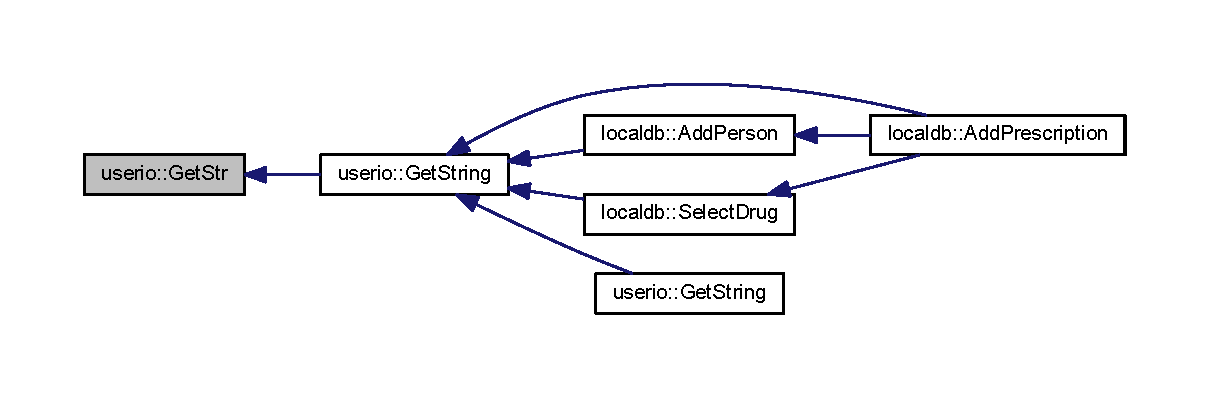
\includegraphics[width=350pt]{dc/ddf/classuserio_a4bcb13a6da031a044765003a310b9df5_icgraph}
\end{center}
\end{figure}


\hypertarget{classuserio_ae31f1f0b7982933a8c9ac5ac683b7450}{\index{userio@{userio}!Get\-String@{Get\-String}}
\index{Get\-String@{Get\-String}!userio@{userio}}
\subsubsection[{Get\-String}]{\setlength{\rightskip}{0pt plus 5cm}std\-::string userio\-::\-Get\-String (
\begin{DoxyParamCaption}
\item[{std\-::string}]{pre, }
\item[{int}]{how, }
\item[{std\-::string}]{str1 = {\ttfamily \char`\"{}\char`\"{}}, }
\item[{const int}]{min = {\ttfamily 0}, }
\item[{unsigned const int}]{max = {\ttfamily 0}}
\end{DoxyParamCaption}
)\hspace{0.3cm}{\ttfamily [static]}}}\label{dc/ddf/classuserio_ae31f1f0b7982933a8c9ac5ac683b7450}
Sanitizes a string (as determined by the interaction enum 'how')


\begin{DoxyParams}{Parameters}
{\em string} & pre Text to print before catching users input \\
\hline
{\em integer} & how Determines how the expected integer should be \\
\hline
{\em int} & str1 Used when 'how' is not set to N\-O\-F\-I\-L\-T\-E\-R to compare against \\
\hline
{\em int} & min Used when how is set to M\-I\-N or B\-E\-T\-W\-E\-E\-N \\
\hline
{\em int} & max Used when how is set to M\-A\-X or B\-E\-T\-W\-E\-E\-N \\
\hline
\end{DoxyParams}
\begin{DoxyReturn}{Returns}
string 
\end{DoxyReturn}


Here is the call graph for this function\-:\nopagebreak
\begin{figure}[H]
\begin{center}
\leavevmode
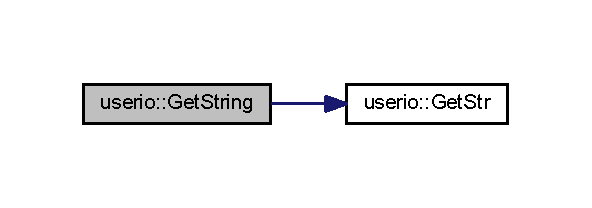
\includegraphics[width=284pt]{dc/ddf/classuserio_ae31f1f0b7982933a8c9ac5ac683b7450_cgraph}
\end{center}
\end{figure}




Here is the caller graph for this function\-:\nopagebreak
\begin{figure}[H]
\begin{center}
\leavevmode
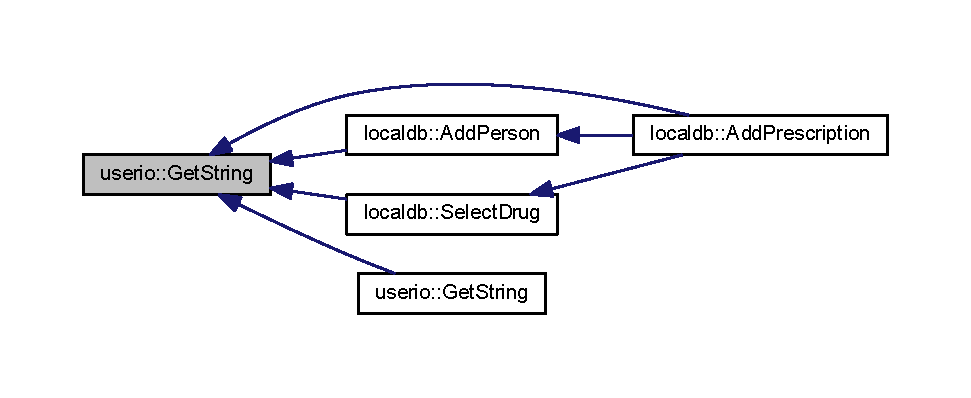
\includegraphics[width=350pt]{dc/ddf/classuserio_ae31f1f0b7982933a8c9ac5ac683b7450_icgraph}
\end{center}
\end{figure}


\hypertarget{classuserio_a8cce5c74bcb42130d51d28dca9cca56c}{\index{userio@{userio}!Get\-String@{Get\-String}}
\index{Get\-String@{Get\-String}!userio@{userio}}
\subsubsection[{Get\-String}]{\setlength{\rightskip}{0pt plus 5cm}std\-::string userio\-::\-Get\-String (
\begin{DoxyParamCaption}
\item[{std\-::string}]{pre, }
\item[{std\-::string}]{regex, }
\item[{std\-::string}]{readable\-\_\-regex}
\end{DoxyParamCaption}
)\hspace{0.3cm}{\ttfamily [static]}}}\label{dc/ddf/classuserio_a8cce5c74bcb42130d51d28dca9cca56c}
Gets a string from the user through the input stream only if it matches the specified regex pattern.


\begin{DoxyParams}{Parameters}
{\em string} & pre \\
\hline
{\em string} & regex \\
\hline
\end{DoxyParams}
\begin{DoxyReturn}{Returns}
string 
\end{DoxyReturn}


Here is the call graph for this function\-:\nopagebreak
\begin{figure}[H]
\begin{center}
\leavevmode
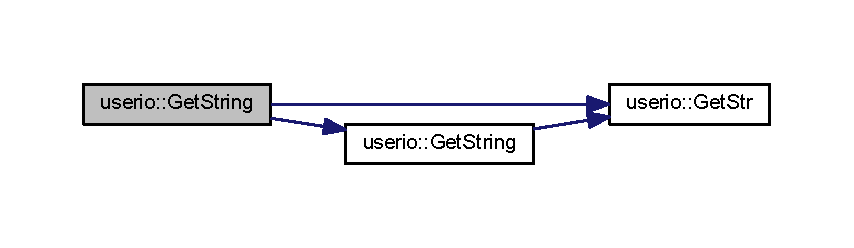
\includegraphics[width=350pt]{dc/ddf/classuserio_a8cce5c74bcb42130d51d28dca9cca56c_cgraph}
\end{center}
\end{figure}


\hypertarget{classuserio_ad89aefb694383c172e04af7efb2a96fa}{\index{userio@{userio}!Get\-Time@{Get\-Time}}
\index{Get\-Time@{Get\-Time}!userio@{userio}}
\subsubsection[{Get\-Time}]{\setlength{\rightskip}{0pt plus 5cm}struct tm userio\-::\-Get\-Time (
\begin{DoxyParamCaption}
\item[{std\-::string}]{pre}
\end{DoxyParamCaption}
)\hspace{0.3cm}{\ttfamily [static]}, {\ttfamily [read]}}}\label{dc/ddf/classuserio_ad89aefb694383c172e04af7efb2a96fa}
Creates a timestruct from userprovided hour and time.


\begin{DoxyParams}{Parameters}
{\em string} & pre Pretext to show before taking input \\
\hline
\end{DoxyParams}
\begin{DoxyReturn}{Returns}
struct tm 
\end{DoxyReturn}


Here is the caller graph for this function\-:\nopagebreak
\begin{figure}[H]
\begin{center}
\leavevmode
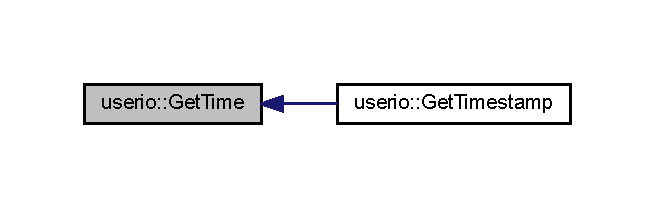
\includegraphics[width=314pt]{dc/ddf/classuserio_ad89aefb694383c172e04af7efb2a96fa_icgraph}
\end{center}
\end{figure}


\hypertarget{classuserio_ad764988b25a5491ff4d09f096aaa3e36}{\index{userio@{userio}!Get\-Timestamp@{Get\-Timestamp}}
\index{Get\-Timestamp@{Get\-Timestamp}!userio@{userio}}
\subsubsection[{Get\-Timestamp}]{\setlength{\rightskip}{0pt plus 5cm}time\-\_\-t userio\-::\-Get\-Timestamp (
\begin{DoxyParamCaption}
\item[{std\-::string}]{pre}
\end{DoxyParamCaption}
)\hspace{0.3cm}{\ttfamily [static]}}}\label{dc/ddf/classuserio_ad764988b25a5491ff4d09f096aaa3e36}
Creates requests date and time from user, and returns timestamp


\begin{DoxyParams}{Parameters}
{\em string} & pre Pretext to show before taking input \\
\hline
\end{DoxyParams}
\begin{DoxyReturn}{Returns}
time\-\_\-t 
\end{DoxyReturn}


Here is the call graph for this function\-:\nopagebreak
\begin{figure}[H]
\begin{center}
\leavevmode
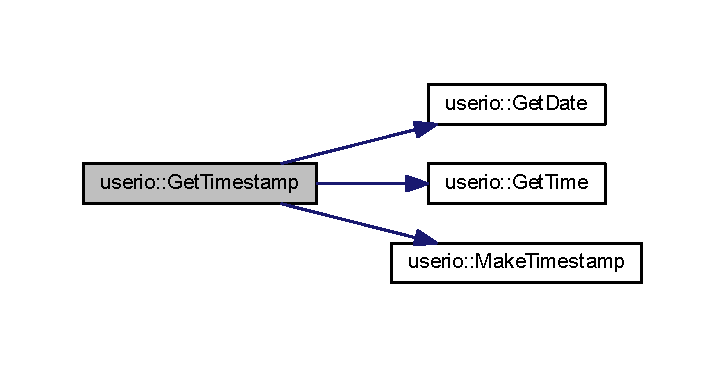
\includegraphics[width=348pt]{dc/ddf/classuserio_ad764988b25a5491ff4d09f096aaa3e36_cgraph}
\end{center}
\end{figure}


\hypertarget{classuserio_a815f7bcecc23024e5b2e7a2584f13222}{\index{userio@{userio}!Make\-Timestamp@{Make\-Timestamp}}
\index{Make\-Timestamp@{Make\-Timestamp}!userio@{userio}}
\subsubsection[{Make\-Timestamp}]{\setlength{\rightskip}{0pt plus 5cm}time\-\_\-t userio\-::\-Make\-Timestamp (
\begin{DoxyParamCaption}
\item[{struct tm}]{clock, }
\item[{struct tm}]{date}
\end{DoxyParamCaption}
)\hspace{0.3cm}{\ttfamily [static]}}}\label{dc/ddf/classuserio_a815f7bcecc23024e5b2e7a2584f13222}
Merges time and date from two different tm structs


\begin{DoxyParams}{Parameters}
{\em struct} & tm clock Time struct \\
\hline
{\em struct} & tm date Date struct \\
\hline
\end{DoxyParams}
\begin{DoxyReturn}{Returns}
time\-\_\-t 
\end{DoxyReturn}


Here is the caller graph for this function\-:\nopagebreak
\begin{figure}[H]
\begin{center}
\leavevmode
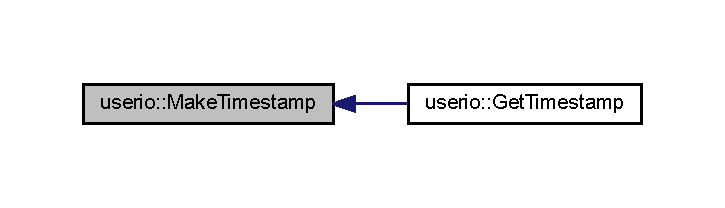
\includegraphics[width=348pt]{dc/ddf/classuserio_a815f7bcecc23024e5b2e7a2584f13222_icgraph}
\end{center}
\end{figure}




The documentation for this class was generated from the following files\-:\begin{DoxyCompactItemize}
\item 
userio.\-h\item 
userio.\-cpp\end{DoxyCompactItemize}

\addcontentsline{toc}{part}{Index}
\printindex
\end{document}
